\section{紧致曲面的构造}
\label{ch12-sec78}

为完成紧致曲面的分类, 必须证明每一个紧致连通曲面都可以通过成对地黏合多边形区域的边的方式获得. 事实上, 我们将证明比这稍弱一点的结论, 因为我们将假设所涉及的曲面有一个三角剖分. 定义这个概念如下.

\begin{definition}[弯曲的三角形与三角剖分]
\label{definition:ch12-triangulation}
设 $X$ 是一个紧致的 Hausdorff 空间. $X$ 中的一个\textbf{弯曲的三角形}(curved triangle)是指 $X$ 的一个子空间 $A$ 和一个同胚 $h\colon T\to A$, 其中 $T$ 是平面上的一个闭的三角形区域. 若 $e$ 为 $T$ 的一条边, 则称 $h(e)$ 为 $A$ 的一条\textbf{边}(edge). 若 $v$ 为 $T$ 的一个顶点, 则称 $h(v)$ 为 $A$ 的一个顶点(vertex). $X$ 的一个\textbf{三角剖分}(triangulation)是 $X$ 中的弯曲的三角形的一个族 $A_{1},\ \cdots,\ A_{n}$, 它们的并为 $X$, 并且当 $i\neq j$ 时, $A_{i}\cap A_{j}$ 或者是空集, 或者是 $A_{i}$ 和 $A_{j}$ 的公共顶点, 或者是两者的公共边. 此外, 设 $h_{i}\colon T_{i}\to A_{i}$ 为相应于 $A_{i}$ 的同胚, 当 $A_{i}\cap A_{j}$ 为它们的一个公共边 $e$ 时, 我们要求映射 $h_{j}^{-1}h_{i}$ 是 $T_{i}$ 的边 $h_{i}^{-1}(e)$ 与 $T_{j}$ 的边 $h_{j}^{-1}(e)$ 之间的一个线性同胚. 如果 $X$ 有一个三角剖分, 我们称它是\textbf{可三角剖分的}(triangulable).
\end{definition}

有一个基本定理: 每一个紧致曲面都可三角剖分. 这个定理的证明较长, 但并不十分困难 (参见 [A-S] 或 [D-M]).

\begin{theorem}[可三角剖分曲面的商表示]
\label{theorem:ch12-triangulable-quotient}
若 $X$ 为可三角剖分的紧致曲面, 则 $X$ 同胚于平面上两两无交的三角形区域的一个族通过成对地黏合边而得到的一个商空间.
\end{theorem}

\par
\begin{figure}[htbp]
\centering
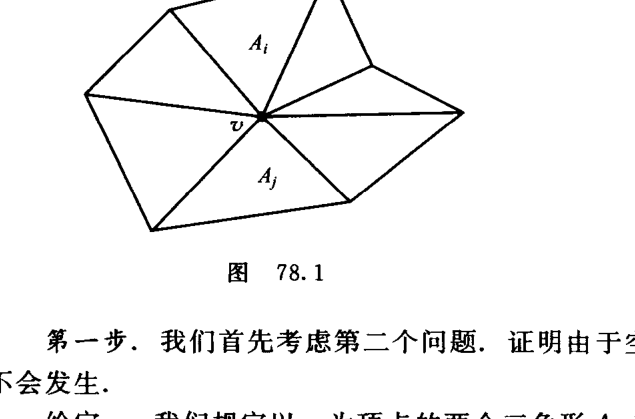
\includegraphics[width=0.45\textwidth]{image/fig-78-1.png}
\caption{环绕顶点 $v$ 的三角形序列.}
\label{ch12-fig-78-1}
\end{figure}

\par
\begin{figure}[htbp]
\centering
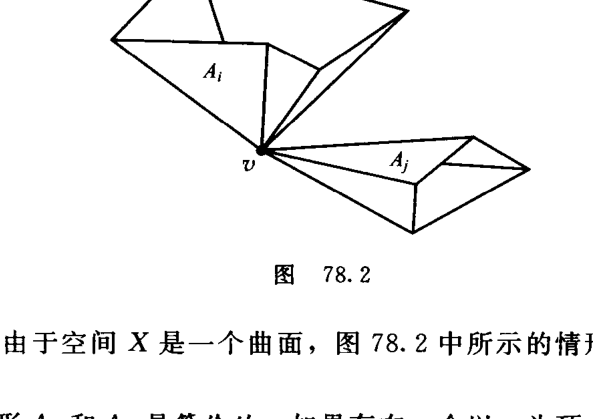
\includegraphics[width=0.45\textwidth]{image/fig-78-2.png}
\caption{不希望出现的情形.}
\label{ch12-fig-78-2}
\end{figure}

\par
\begin{figure}[htbp]
\centering
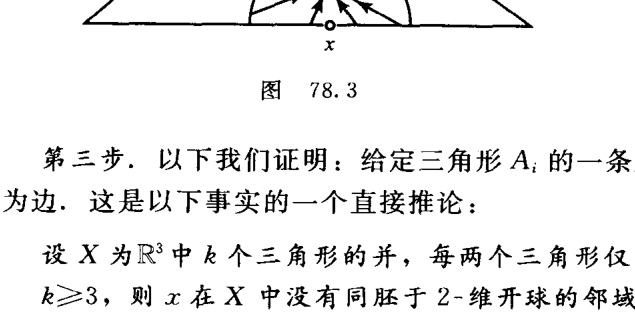
\includegraphics[width=0.45\textwidth]{image/fig-78-3.png}
\caption{边的内点 $x$ 的邻域.}
\label{ch12-fig-78-3}
\end{figure}

\par
\begin{figure}[htbp]
\centering
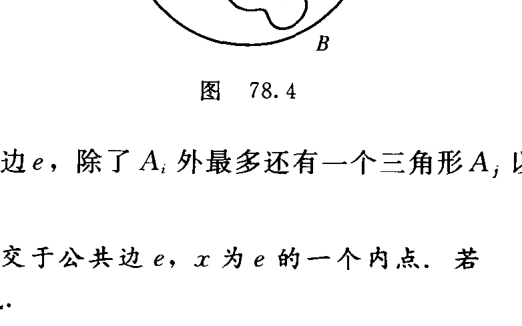
\includegraphics[width=0.4\textwidth]{image/fig-78-4.png}
\caption{$V-0$ 不是单连通的.}
\label{ch12-fig-78-4}
\end{figure}

\par
\begin{figure}[htbp]
\centering
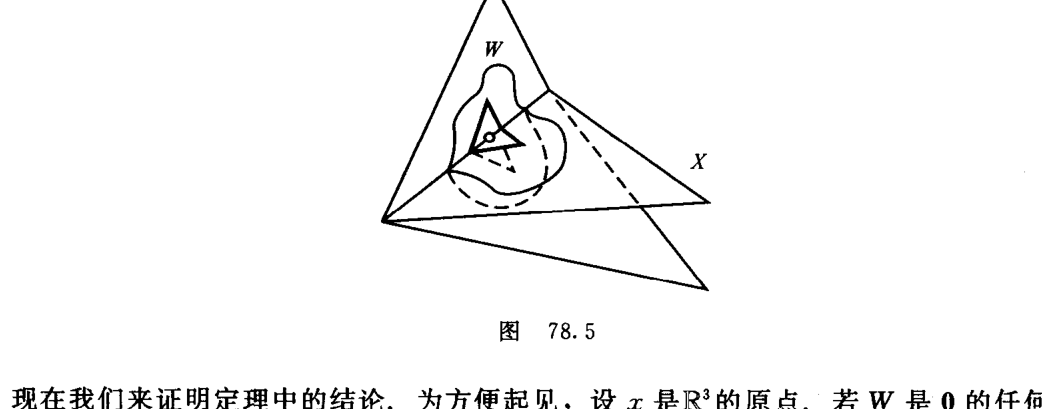
\includegraphics[width=0.6\textwidth]{image/fig-78-5.png}
\caption{$X-x$ 的基本群不是阿贝尔群.}
\label{ch12-fig-78-5}
\end{figure}

\begin{proof}
设 $A_{1},\ \cdots,\ A_{n}$ 是 $X$ 上的一个三角剖分, 其相应的同胚为 $h_{i}\colon T_{i}\to A_{i}$. 假定诸三角形 $T_{i}$ 是两两无交的, 则诸映射 $h_{i}$ 拼合在一起定义了一个商映射 $h\colon E=T_{1}\cup\cdots\cup T_{n}\to X$ (因为 $E$ 是紧致的且 $X$ 是一个 Hausdorff 空间). 进而, 当 $A_{i}$ 与 $A_{j}$ 相交于它们的公共边时, 由于映射 $h_{j}^{-1}\circ h_{i}$ 是线性的, 所以 $h$ 将 $T_{i}$ 与 $T_{j}$ 的边经一个线性同胚黏合.

我们需要证明两个结论. 第一, 必须证明对于一个三角形 $A_{i}$ 的每一条边 $e$, 恰好有另一个三角形 $A_{j}$ 使得 $A_{i}\cap A_{j}=e$. 这意味着商映射 $h$ 成对地黏合诸三角形 $T_{i}$ 的边.

第二个结论则很不明显. 我们必须证明: 如果交 $A_{i}\cap A_{j}$ 是两个三角形的公共顶点 $v$, 则存在一系列三角形以 $v$ 为顶点, 这一系列三角形从 $A_{i}$ 开始到 $A_{j}$ 结束, 其中每相邻的两个三角形都相交于一条公共边. 参见\cref{ch12-fig-78-1}.

如果不顾及这一点, 可能出现\cref{ch12-fig-78-2} 中所示的情形. 此时我们不能仅通过诸三角形 $T_{i}$ 的各边的黏合方式来定义商映射 $h$, 当边的黏合方式并不能确定顶点的黏合方式时, 我们还必须指定顶点的黏合方式.



\textbf{第一步.} 我们首先考虑第二个问题. 证明由于空间 $X$ 是一个曲面, \cref{ch12-fig-78-2} 中所示的情形不会发生.

给定 $v$, 我们规定以 $v$ 为顶点的两个三角形 $A_{i}$ 和 $A_{j}$ 是等价的, 如果存在一个以 $v$ 为顶点的三角形序列, 从 $A_{i}$ 开始到 $A_{j}$ 结束, 并且这个序列中的每一个三角形与其后面接着的那个三角形的交是这两个三角形的公共边. 如果等价类多于一个, 设 $B$ 是某一个等价类中的所有三角形的并, $C$ 是另一等价类中的所有三角形的并. 由于 $B$ 中的任何一个三角形与 $C$ 中的任何一个三角形没有公共边, 从而 $B$ 与 $C$ 的交是一个顶点 $v$. 由此可见, 对于点 $v$ 在 $X$ 中的任何一个充分小的邻域 $W$, $W-v$ 不连通.

另一方面, 如果 $X$ 是一个曲面, 那么 $v$ 有一个同胚于 $2$-维开球的邻域. 因此, 对于 $v$ 的任意小的邻域 $W$, $W-v$ 是连通的.

\textbf{第二步.} 我们再来处理第一个结论. 它略为繁琐些. 首先我们来证明: 对于任意给定的一个以 $e$ 为边的三角形 $A_{i}$, 至少有一个异于 $A_{i}$ 的三角形 $A_{j}$ 也以 $e$ 为边. 这是以下结论的一个推论:

\begin{quote}
设 $X$ 是平面上的一个三角形区域, $x$ 为 $X$ 的某条边的内点, 则 $x$ 在 $X$ 中没有同胚于 $2$-维开球的邻域.
\end{quote}

为证明此结论, 注意 $x$ 有任意小的邻域 $W$ 使得 $W-x$ 是单连通的. 事实上, 如果 $W$ 是 $x$ 在 $X$ 中的 $\varepsilon$ 邻域, 对于充分小的 $\varepsilon$, $W-x$ 可以缩成一点. 参见\cref{ch12-fig-78-3}.

另一方面, 假设 $x$ 有同胚于 $\mathbb{R}^{2}$ 中的某开球的一个邻域 $U$, 其中的一个同胚将 $x$ 映为 $0$. 我们将证明 $x$ 没有任意小的邻域 $W$ 使得 $W-x$ 是单连通的.

事实上, 设 $B$ 是 $\mathbb{R}^{2}$ 中以原点为圆心的开球, 并设 $V$ 是 $0$ 包含于 $B$ 中的任何一个邻域. 选取 $\varepsilon$ 使得以 $0$ 为圆心、以 $\varepsilon$ 为半径的开球 $B_{\varepsilon}$ 包含于 $V$ 中, 并且考虑内射构成的图
\[
B_{\varepsilon}-0\longrightarrow B-0,
\]
其中 $B_{\varepsilon}-0\to V-0\to B-0$. 内射 $i$ 同伦于同胚 $h(x)=x/\varepsilon$, 从而它诱导了基本群之间的一个同构. 因此, $k_{*}$ 是一个满射, 因而 $V-0$ 不是单连通的. 参见\cref{ch12-fig-78-4}.



\textbf{第三步.} 以下我们证明: 给定三角形 $A_{i}$ 的一条边 $e$, 除了 $A_{i}$ 外最多还有一个三角形 $A_{j}$ 以 $e$ 为边. 这是以下事实的一个直接推论:

\begin{quote}
设 $X$ 为 $\mathbb{R}^{3}$ 中 $k$ 个三角形的并, 每两个三角形仅交于公共边 $e$, $x$ 为 $e$ 的一个内点. 若 $k\geqslant 3$, 则 $x$ 在 $X$ 中没有同胚于 $2$-维开球的邻域.
\end{quote}

我们证明: 不存在 $x$ 在 $X$ 中的邻域 $W$, 使得 $W-x$ 的基本群是阿贝尔群. 由此推得 $x$ 没有同胚于 $2$-维开球的邻域.

首先证明: 若 $A$ 是 $X$ 中的三角形的所有异于 $e$ 的边的并, 则 $A$ 的基本群不是一个阿贝尔群. 空间 $A$ 是 $k$ 条弧的并, 每两条仅交于端点. 如果 $B$ 是构成 $A$ 的那些弧中某三条弧的并, 则存在一个从 $A$ 到 $B$ 上的收缩 $r$, 它将所有不在 $B$ 中的那些弧同胚地映到 $B$ 中的某条弧上, 并且保持端点不动. 于是 $r_{*}$ 是一个满同态. 由于 $B$ 的基本群不是阿贝尔群 (根据第 70 节的例 1 或第 58 节的例 3), 所以 $A$ 的基本群也不是阿贝尔群.

易见, 由于 $A$ 是 $X-x$ 的一个形变收缩, 因此 $X-x$ 的基本群也不是阿贝尔群. 见\cref{ch12-fig-78-5}.


现在我们来证明定理中的结论. 为方便起见, 设 $x$ 是 $\mathbb{R}^{3}$ 的原点. 若 $W$ 是 $0$ 的任何一个邻域, 我们有一个"收缩" $f(x)=\varepsilon x$ 将 $X$ 映入 $W$ 中. 空间 $X_{\varepsilon}=f(X)$ 是 $X$ 在 $W$ 内部的一个拷贝. 考虑内射构成的图 $X_{\varepsilon}-0\to X-0$ 经由 $W-0$. 内射 $i$ 同伦于同胚 $h(x)=x/\varepsilon$, 因此它诱导基本群之间的一个同构. 从而 $k_{*}$ 是一个满射, 于是 $W-0$ 的基本群不是阿贝尔群.
\end{proof}

\begin{theorem}[紧致连通曲面的多边形表示]
\label{theorem:ch12-polygon-representation}
若 $X$ 是一个可三角剖分的紧致连通曲面, 则 $X$ 同胚于一个成对地黏合某平面多边形区域的边所得到的空间.
\end{theorem}

\begin{proof}
根据前一个定理可见, 平面上有三角形区域的一个族 $T_{1},\ \cdots,\ T_{n}$, 并且对这些三角形区域的每一条边给了一个定向和一个标记, 其中每一个标签在全部标记表中正好出现两次, 并且使得 $X$ 同胚于通过这些区域借助于这个标记表得到的商空间.

我们应用第 76 节中给出的黏合运算. 若两个三角形区域含有使用同一标签的边, 我们便沿这个边将两个区域黏合 (必要时, 先对一个区域应用翻转运算). 其结果是将两个三角形区域变成一个 $4$-边形区域, 并且这个新区域的各条边保持着先前的定向和标记. 继续类似的做法, 只要还存在两个区域, 它们有边具有相同的标签, 便可以将它们黏合.

最终会出现两种情形, 其一是获得一个多边形区域, 此时定理成立. 其二是得到几个多边形区域, 两两间不再有相同的标签的边. 这说明上述所进行的边的黏合得到的空间是不连通的. 事实上, 每一个区域给出这个空间的一个连通分支. 由于 $X$ 是连通的, 所以这种情形不会出现.
\end{proof}

\begin{exercise}
\label{exercise:ch12-sec78-01}
以下每一组 $4$ 个三角形区域上的标记表确定的是何种空间?
\begin{enumerate}[(a)]
\item $abc$, $dae$, $bef$, $cdf$.
\item $abc$, $cba$, $def$, $dfe^{-1}$.
\end{enumerate}
\end{exercise}

\begin{exercise}
\label{exercise:ch12-sec78-02}
设 $H^{2}$ 是由 $\mathbb{R}^{2}$ 中所有满足 $x_{2}\geqslant 0$ 的点 $(x_{1},\ x_{2})$ 所构成的子空间. 一个\textbf{带边的 $2$-维流形}(或者, 带边曲面)是一个有可数基的 Hausdorff 空间 $X$, 使得 $X$ 中每一点 $x$ 都有一个邻域同胚于 $\mathbb{R}^{2}$ 或 $H^{2}$ 的一个开集. $X$ 的\textbf{边界}(boundary)(记作 $\partial X$)是由 $X$ 中那些没有邻域同胚于 $\mathbb{R}^{2}$ 中的开集的那些点 $x$ 组成的集合.
\begin{enumerate}[(a)]
\item 证明 $H^{2}$ 中所有形如 $(x_{1},\ 0)$ 的点 (在 $H^{2}$ 中) 都没有同胚于 $\mathbb{R}^{2}$ 中的开集的邻域.
\item 证明 $x\in\partial X$ 当且仅当存在一个从 $x$ 的一个邻域到 $H^{2}$ 中的一个开集的同胚 $h$, 使得 $h(x)\in\mathbb{R}\times 0$.
\item 证明 $\partial X$ 是一个 $1$-维流形.
\end{enumerate}
\end{exercise}

\begin{exercise}
\label{exercise:ch12-sec78-03}
证明 $\mathbb{R}^{2}$ 中的闭单位球是一个带边的 $2$-维流形.
\end{exercise}

\begin{exercise}
\label{exercise:ch12-sec78-04}
设 $X$ 是一个 $2$-维流形, $U_{1},\ \cdots,\ U_{k}$ 是 $X$ 中无交开集的一个族. 假定对于每一个 $i$, 存在开单位球 $B^{2}$ 与 $U_{i}$ 之间的一个同胚 $h_{i}$. 设 $\varepsilon=1/2$ 以及 $B_{\varepsilon}$ 是半径为 $\varepsilon$ 的开球. 证明空间 $Y=X-\bigcup h_{i}(B_{\varepsilon})$ 是一个带边的 $2$-维流形, 并且 $\partial Y$ 有 $k$ 个分支. 空间 $Y$ 叫做有 $k$ 个洞的 $X$.
\end{exercise}

\begin{exercise}
\label{exercise:ch12-sec78-05}
证明以下定理:

\begin{theorem}[带边曲面的分类]
\label{theorem:ch12-bordered-classification}
给定一个可三角剖分的紧致连通的带边 $2$-维流形 $Y$, 使得 $\partial Y$ 有 $k$ 个分支, 那么 $Y$ 同胚于有 $k$ 个洞孔的 $X$, 其中 $X$ 是 $S^{2}$、$n$-重环面 $T_{n}$ 或者 $m$-重射影平面 $P_{m}$.
\end{theorem}
[提示: $\partial Y$ 的每一个分支同胚于圆周.]
\end{exercise}
